% 
%            ,,                                        
%          `7MM            _.o9                                
%            MM                                             
%  ,6"Yb.    MM  ,p6"bo   ,6"Yb.  M"""MMV  ,6"Yb.  `7Mb,od8 
% 8)   MM    MM 6M'  OO  8)   MM  '  AMV  8)   MM    MM' "' 
%  ,pm9MM    MM 8M        ,pm9MM    AMV    ,pm9MM    MM     
% 8M   MM    MM YM.    , 8M   MM   AMV  , 8M   MM    MM     
% `Moo9^Yo..JMML.YMbmd'  `Moo9^Yo.AMMmmmM `Moo9^Yo..JMML.   
% 
% 
% Free and Open-Source template for academic works
% https://github.com/dpmj/alca



\clearpage
\cleardoublepage

\chapter{Introduzione}

Questa tesi di laurea ha l'obiettivo di evidenziare le potenzialità di Kubernetes e dell'approccio distribuito ai problemi di Machine Learning, definendo una struttura concreta e organica per implementare pipeline completamente gestite ({\em "fully-managed"}) relative all'intero ciclo di vita dei modelli di machine learning. Verrà proposta un'analisi compilativa dello stato dell'arte strettamente correlato a questo contesto tecnologico, proponendo un contributo sperimentale legato alla trasformazione in microservizi di modelli monolitici pre-esistenti; successivamente, si esibirà un'analisi ad ampio spettro delle possibili vulnerabilità dell'architettura realizzata, fornendo anche in questo caso un contributo originale circa l'implementazione containerizzata di strumenti di attacco e ambienti vulnerabili.

Nel secondo capitolo, si presenterà un problema bioinformatico ad alta complessità relativo all'analisi genomica e alla classificazione dei geni di fusione, per i quali sono stati realizzati - nel contesto di altre tesi magistrali - due modelli di machine learning declinati in architetture monolitiche. Si descriveranno dunque le caratteristiche e il funzionamento a basso ed alto livello dei due modelli, evidenziando i difetti della loro attuale architettura.

Nel terzo capitolo, si delineeranno con formalità e precisione le tecnologie e gli strumenti informatici impiegati nei contesti distribuiti di Machine Learning. Si definiranno le principali convenzioni coinvolte, come le architetture a microservizi, e i concetti di orchestrazione, containerizzazione e virtualizzazione. Si descriveranno strumenti specifici finalizzati all'orchestrazione di generici carichi di lavoro, come \glsname{kubernetes}, proponendo poi anche uno strumento specifico ai carichi di Machine Learning, quale \glsname{kubeflow}. Si analizzeranno le architetture a basso livello di ambo le tecnologie per comprenderne a pieno le funzionalità, discutendo inoltre di come poter iterare sulle medesime attraverso lo sviluppo di componenti e pipeline di Machine Learning ex novo. Si accennerà brevemente a possibili alternative a Kubeflow, come \glsname{mxnet}, \glsname{ray} e \glsname{mlflow}, nonché ad alcuni possibili provider di cloud computing (\glsname{aws}, \glsname{gcp}) che offrono servizi completamente gestiti per i cluster Kubernetes.

Nel quarto capitolo, i modelli descritti nel secondo capitolo subiranno una trasformazione in microservizi così come proposto nel terzo capitolo, sfruttando Kubernetes e Kubeflow per lo sviluppo delle pipeline distribuite. L'intero processo, opportunamento documentato, esibirà le sue potenzialità in un benchmark delle prestazioni, rilevando un miglioramento notevole dei tempi di esecuzione. Inoltre, si delineeranno le modalità di integrazione di driver CUDA per l'utilizzo della GPU nelle fasi di training e testing, e il funzionamento di registry di immagini Docker on-premise.

Nel quinto capitolo, si avanzeranno una serie di considerazioni compilative e sperimentali di \glsname{mlsecops}. In particolare, veranno impiegate tecnologie allo stato dell'arte, come \glsname{metasploit}, \glsname{kali}, \glsname{cdk} e \glsname{artillery}, per tarare e penetrare le difese dell'infrastruttura realizzata, esponendone vulnerabilità per poi mitigare i rischi di intrusione. Sono inoltre proposti ulteriori contributi sperimentali, contestuali a questo lavoro di tesi, circa la produzione di immagini Docker degli strumenti indicati. 

Nel sesto capitolo, vengono delineati i possibili sviluppi futuri che potrebbero permette di traslare in produzione l'infrastruttura presentata. In particolare, si accenna alla possibilità di integrare tecniche di \glsname{mlre} e \glsname{datagovernance} per amplificare la sicurezza e resilienza del sistema; inoltre, si individua in \glsname{helm} una possibile modalità di distribuzione dell'architettura come applicazione Kubernetes portabile.

\section{La Rivoluzione DevOps e le sue conseguenze}

Il Movimento \glsname{devops}, nato dalla convergenza tra "development" e "operations", si è delineato come risposta alle sfide emergenti nel ciclo di vita dello sviluppo del software. Il suo percorso evolutivo può essere tracciato attraverso una serie di fasi che hanno modellato e influenzato la sua crescita.

\begin{figure}[h]
    \centering
    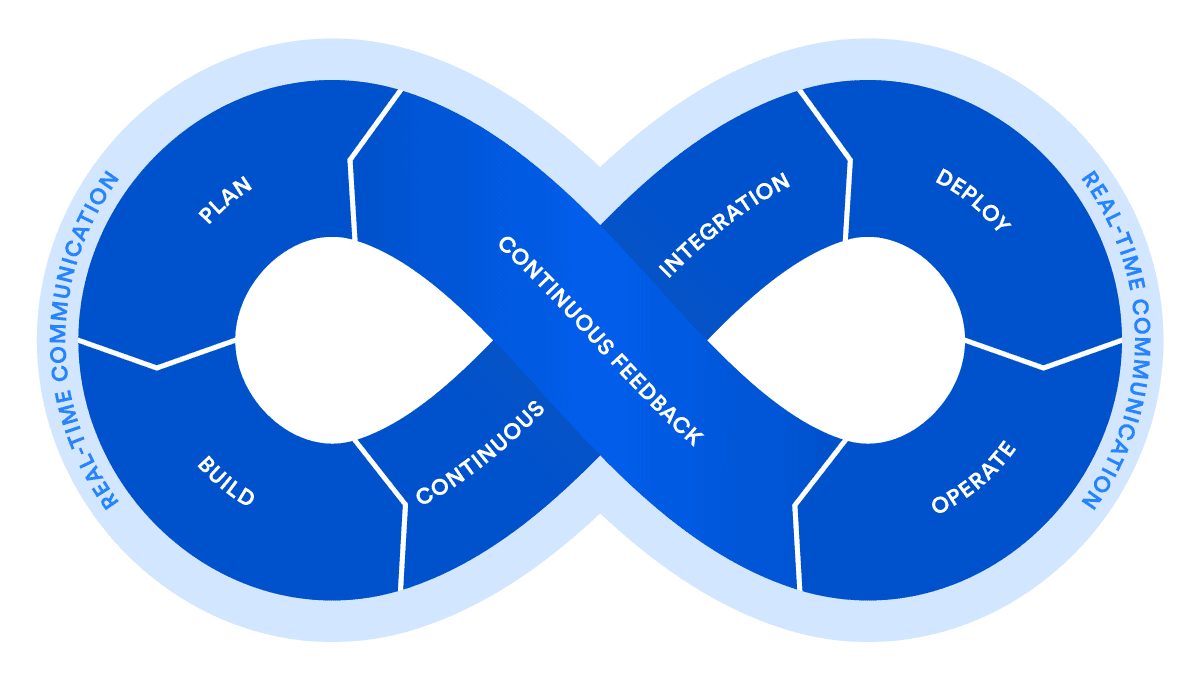
\includegraphics[width=200px]{figures/ch1/devops-flow.png}
    \caption[Development \& Operations: un'icona del movimento DevOps]{Development \& Operations: un'icona del movimento DevOps}
    \label{fig:cha1:devops}
\end{figure}

Negli anni 2000, le crescenti complessità delle applicazioni e la necessità di cicli di rilascio più rapidi hanno reso evidente la necessità di una collaborazione più stretta tra team di sviluppo e team operativo, inteso come l'insieme di tecnici e ingegneri dediti alla distribuzione delle applicazioni e al mantenimento delle pipeline di rilascio. Questo periodo ha visto la formazione di una consapevolezza crescente dell'importanza di superare le barriere tradizionali tra queste due squadre distinte.

\begin{figure}[h]
    \centering
    \subfloat["The Phoenix Project" (2013)]["The Phoenix Project" (2013)]{
        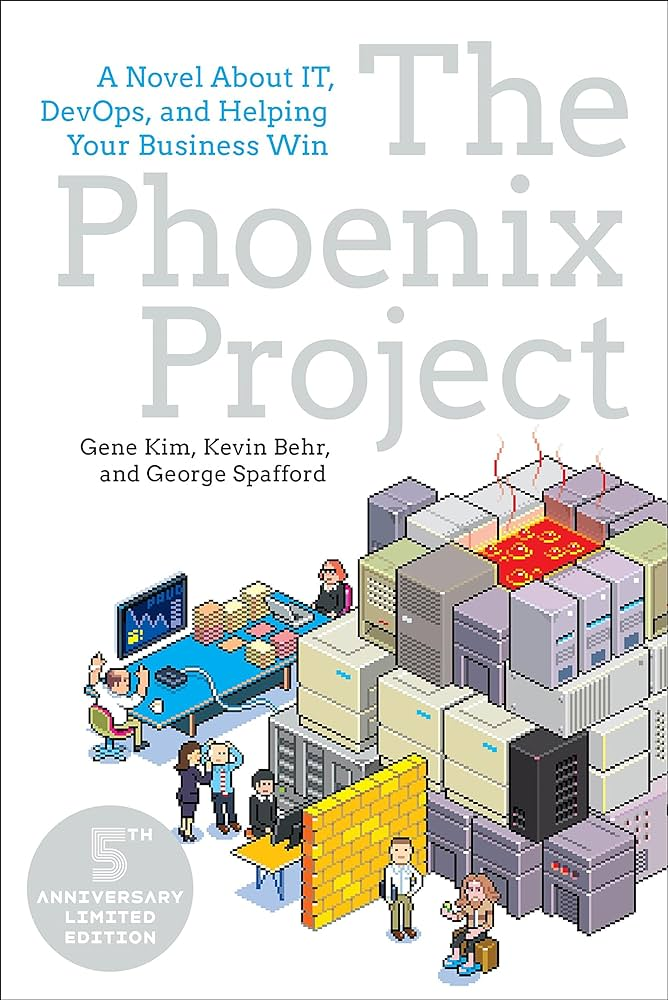
\includegraphics[width=150px]{figures/ch1/phoenix_project.jpg}
            \label{fig:cha1:unicorn}
    }
    \hspace{30px}
    \subfloat["The Unicorn Project" (2019)]["The Unicorn Project" (2019)]{
        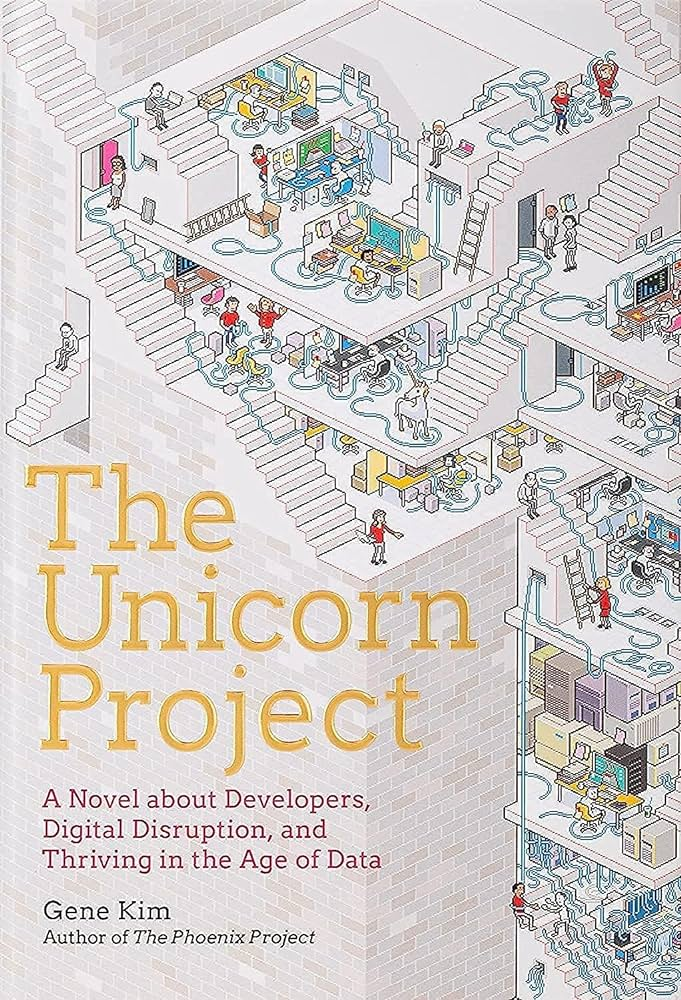
\includegraphics[width=150px]{figures/ch1/unicorn_project.jpg}
            \label{fig:cha1:phoenix}
    }
    \caption{Copertine di "The Phoenix Project" e "The Unicorn Project"}
    \label{fig:cha1:jerez}
\end{figure}

Il termine "{\em DevOps}" è stato coniato nel 2009 durante una conferenza a Bruxelles, segnando un punto di svolta nel modo in cui le organizzazioni affrontano le sfide della distribuzione software. Patrick Debois e Andrew Shafer sono stati tra i pionieri di questa iniziativa, cercando di superare i conflitti tra sviluppatori e operatori.

Negli anni successivi, il Movimento DevOps ha iniziato a focalizzarsi sulla definizione di pratiche e principi chiave, con l'obiettivo di migliorare la collaborazione, la trasparenza e la velocità di rilascio. Il libro "The Phoenix Project" \cite{phoenix} di Gene Kim, Kevin Behr e George Spafford (2013) ha contribuito a diffondere i concetti fondamentali del movimento DevOps, enfatizzando la cultura ingegneristica, l'automazione, la misurazione delle performance e il miglioramento continuo delle competenze (CALMS).

La diffusione del movimento DevOps è stata accompagnata dall'adozione di strumenti e pratiche di automazione. Strumenti come Puppet, Chef e Ansible hanno semplificato la gestione delle configurazioni, mentre Jenkins ha rivoluzionato la pratica dell'integrazione continua.

Negli ultimi anni, il movimento DevOps è diventato uno standard industriale \cite{devops_1}, adottato da un numero sempre maggiore di organizzazioni. L'integrazione di pratiche DevOps è diventata un requisito chiave per affrontare l'accelerazione della domanda di rilasci software e la necessità di rispondere rapidamente ai cambiamenti del mercato.

L'adozione di pratiche DevOps ha portato a benefici tangibili \cite{devops_2}, come la riduzione dei tempi di rilascio, il miglioramento della qualità del software e un maggiore allineamento tra sviluppo e operazioni. Tuttavia, la complessità nell'implementare con successo DevOps in ambienti eterogenei e la gestione del cambiamento culturale rimangono sfide significative.

\begin{figure}[h]
    \centering
    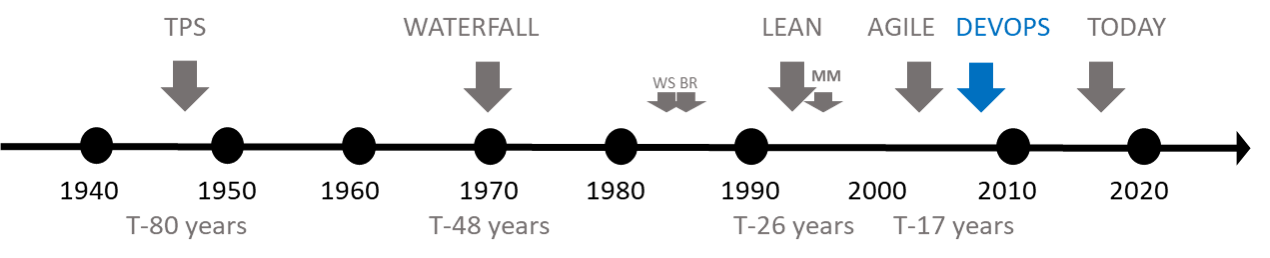
\includegraphics[width=400px]{figures/ch1/devops-timeline.png}
    \caption[Timeline dei metodi di sviluppo nell'industria IT]{Timeline dei metodi di sviluppo nell'industria IT}
    \label{fig:cha1:from_waterfall_to_devops}
\end{figure}

Il Movimento DevOps rappresenta un'evoluzione fondamentale nel modo in cui le organizzazioni affrontano lo sviluppo e il rilascio del software. Dalla sua nascita agli sviluppi recenti, DevOps ha continuato a plasmare il panorama tecnologico e culturale delle aziende, dimostrando la sua essenzialità nell'era della trasformazione digitale.

\section{I paradigmi MLOps e MLSecOps}

Il paradigma \glsname{mlops} ({\em Machine Learning Operations}) e il paradigma \glsname{mlsecops} ({\em Machine Learning Security Operations}) costituiscono una sinergia evolutiva nell'ambito della gestione delle operazioni e della sicurezza nell'implementazione di soluzioni basate su machine learning. Il loro sviluppo è radicato in una cornice storica che riflette l'espansione crescente e la complessità delle applicazioni di intelligenza artificiale (IA) e di machine learning (ML).

\begin{figure}[h]
    \centering
    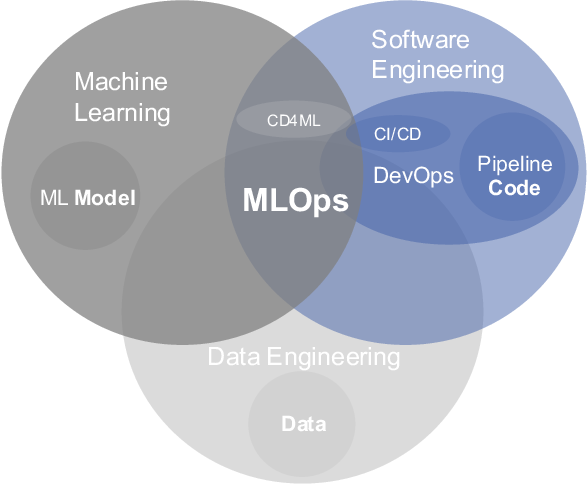
\includegraphics[width=200px]{figures/ch1/mlops-flow.png}
    \caption[Intersezione fra Machine Learning, DevOps e Data Engineering]{Collocamento della branca MLOps nell'informatica}
    \label{fig:cha1:mlops}
\end{figure}

Il paradigma MLOps \cite{mlops} trova le sue radici nella necessità di affrontare le sfide operative emergenti nella gestione di modelli di machine learning su larga scala. Nel corso degli anni, l'adozione di modelli ML è cresciuta esponenzialmente, portando alla comparsa di problemi legati alla distribuzione, all'aggiornamento e al monitoraggio dei modelli in produzione. Il concetto di MLOps ha preso forma attraverso l'esperienza pratica e la risposta alle esigenze operative emergenti nell'industria.

Similmente, il paradigma MLSecOps ha avuto origine dall'urgente necessità di mitigare i rischi legati alla sicurezza nell'ambito dei modelli di machine learning \cite{adv_ml_1}. La crescente consapevolezza delle vulnerabilità specifiche dei modelli ML, come gli attacchi di avversarial machine learning, ha stimolato la nascita di MLSecOps. Questo paradigma mira a integrare le pratiche di sicurezza nell'intero ciclo di vita dei modelli, dalla fase di sviluppo alla fase operativa.

Le motivazioni sottese al paradigma MLOps si concentrano sulla necessità di automatizzare e semplificare il ciclo di vita dei modelli ML, garantendo un deployment efficiente, la gestione delle versioni, il monitoraggio continuo e l'aggiornamento senza intoppi dei modelli in produzione. Il paradigma MLOps si propone di risolvere le sfide operative, garantendo la coerenza tra gli ambienti di sviluppo e produzione, nonché la riproducibilità e la tracciabilità dei risultati.

Dall'altro lato, il paradigma MLSecOps è guidato dalla volontà di proteggere i modelli di machine learning da minacce e attacchi. Ciò implica l'implementazione di misure di sicurezza proattive durante lo sviluppo, nonché la continua valutazione della robustezza dei modelli in produzione. La necessità di comprendere e mitigare le vulnerabilità specifiche dei modelli ML, che possono essere sfruttate da attaccanti astuti, è al centro del paradigma MLSecOps.

I vantaggi del paradigma MLOps sono molteplici e si riflettono nella migliorata efficienza operativa, nella riduzione dei tempi di deployment e nella gestione semplificata delle versioni dei modelli. L'implementazione di pratiche MLOps consente una transizione fluida dai prototipi agli ambienti di produzione, garantendo un flusso di lavoro ottimizzato e una risposta rapida alle esigenze del business.

L'evoluzione del paradigma il paradigma MLOps è strettamente connessa all'avanzamento delle tecnologie che ne supportano l'implementazione. L'adozione di strumenti di automazione, gestione del ciclo di vita e orchestrazione dei modelli ha ridefinito il panorama delle operazioni di machine learning. In particolare, piattaforme come Ray \cite{ray}, MLflow \cite{mlflow} e Kubeflow \cite{kubeflow} hanno svolto un ruolo cruciale nella standardizzazione e semplificazione del flusso di lavoro MLOps.

Tuttavia, è cruciale riconoscere che l'adozione del paradigma MLOps non è esente da sfide. La complessità nell'orchestrare processi di machine learning su vasta scala, la gestione delle dipendenze e la necessità di un monitoraggio continuo possono presentare ostacoli significativi.

Per quanto riguarda il paradigma MLSecOps, i suoi vantaggi sono evidenti nella capacità di proteggere i modelli ML da minacce e attacchi, preservando l'integrità e la riservatezza dei dati. L'integrazione di pratiche di sicurezza fin dalla fase di sviluppo contribuisce a ridurre il rischio di vulnerabilità e garantisce una maggiore fiducia nella robustezza dei modelli.

Le applicazioni del paradigma MLSecOps sono variegate: ad esempio, durante le fasi di sviluppo si potrebbero integrare politiche di data governance; oppure, si potrebbero simulare attacchi mirati contro il modello per identificare vulnerabilità e migliorare la resistenza del sistema. Inoltre, l'implementazione di framework di sicurezza specifici per il machine learning consentirebbe di rilevare e mitigare potenziali minacce come il leaking di dati sensibili o l'inserimento di backdoor nel modello.

Una volta distribuiti, i modelli possono essere protetti attraverso controlli di accesso rigorosi, garantendo che solo utenti autorizzati possano interagire con il sistema. L'implementazione di monitoraggi continui consentirebbe di rilevare anomalie nell'utilizzo del modello, segnalando potenziali attività sospette o tentativi di exploit. Integrando la sicurezza in tutte le fasi del ciclo di vita del modello, dall'addestramento alla distribuzione, sarebbe possibile garantire una protezione efficace contro minacce interne ed esterne, mantenendo la fiducia nell'affidabilità e nella privacy dei modelli di machine learning così costruiti.

Un caso applicativo concreto del paradigma MLSecOps potrebbe riguardare la protezione di un modello di machine learning utilizzato per il rilevamento di malware nei dispositivi IoT all'interno di una rete domestica. Per garantire la sicurezza del modello e dei dati sensibili coinvolti, viene adottato un approccio MLSecOps completo.

Durante la fase di sviluppo del modello, vengono applicate tecniche di robustezza del modello, come descritto da Goodfellow et al. \cite{goodfellow2014explaining}, che includono l'addestramento con dati di addestramento avversariali per rendere il modello più resistente agli attacchi mirati. Inoltre, vengono utilizzati framework di sicurezza specifici per il machine learning, come quello proposto da Papernot et al. \cite{papernot2018deep}, che consentono di rilevare e mitigare potenziali minacce come l'attacco ai dati o l'inserimento di backdoor nel modello.

Una volta distribuito il modello, vengono implementati controlli di accesso rigorosi e monitoraggi continui per proteggere sia il modello stesso che i dati trasferiti e utilizzati durante l'inferenza. Ad esempio, potrebbero essere utilizzati meccanismi di autenticazione e autorizzazione basati su ruoli per garantire che solo utenti autorizzati possano accedere al modello e ai dati. Inoltre, viene applicato un monitoraggio continuo dell'utilizzo del modello, seguendo l'approccio proposto da Laskov et al. \cite{laskov2014practical}, per individuare eventuali anomalie nell'utilizzo che potrebbero indicare un attacco in corso o una compromissione del sistema.

Si osserva che la transizione da paradigma MLOps a MLSecOps è del tutto analoga alla medesima che si ottieni adottando il paradigma DevSecOps a partire da una suite di protocolli e procedure DevOps. Fondamentalmente, la distinzione giace nella natura del carico di lavoro, poiché i paradigmi MLOps e MLSecOps si occupano esclusivamente di carichi di lavoro di machine learning, mentre la metodologia DevSecOps si rifanno a pratiche generalizzabili a una vasta moltitudine di carichi di lavoro.

Tuttavia, anche il paradigma MLSecOps (talvolta citato come SecMLOps) non è immune da sfide \cite{adv_ml_2}. La continua evoluzione delle tecniche di attacco richiede un costante adattamento delle misure di sicurezza, e la complessità degli algoritmi di machine learning può rendere difficile la previsione e la mitigazione di potenziali minacce.

I paradigmi MLOps e MLSecOps rappresentano risposte essenziali alle sfide emergenti nella implementazione di soluzioni di machine learning su larga scala. Mentre l'idea attorno al paradigma MLOps si concentra sull'ottimizzazione delle operazioni di distribuzione di applicativi di machine learning, il paradigma MLSecOps mira a garantire la sicurezza dei modelli di machine learning. L'implementazione sinergica di entrambi i paradigmi può contribuire a un ecosistema ML resiliente e efficiente.